% This section presents the software architecture of Midas. After a brief
% overview, focus is set on NVRAM management, durable data structures, and
% serializable MVCC.

This section presents the software architecture of Midas. After a brief
overview, selected aspects of the implementation, such as durable memory
management, are elaborated in more detail.

Midas is implemented as a C++ library on top of PMDK. PMDK is a set of libraries
for NVRAM management that acts as a middleware between programs using NVRAM and
the underlying system \cite{rudoff2017persistent, pmdk2018home}. As depicted in
Figure \ref{fig:impl-arch}, Midas consists of two components: the key-value
store and a set of durable container structures based on PMDK. The latter are
used to provide the same level of abstraction of conventional containers for
NVRAM. The components of Midas are largely congruent to Figure
\ref{fig:concept-struct-complete} from Section \ref{ch:concept-kvs} and is
described in more detail later in this chapter.

\begin{figure}[h!]
    \centering
    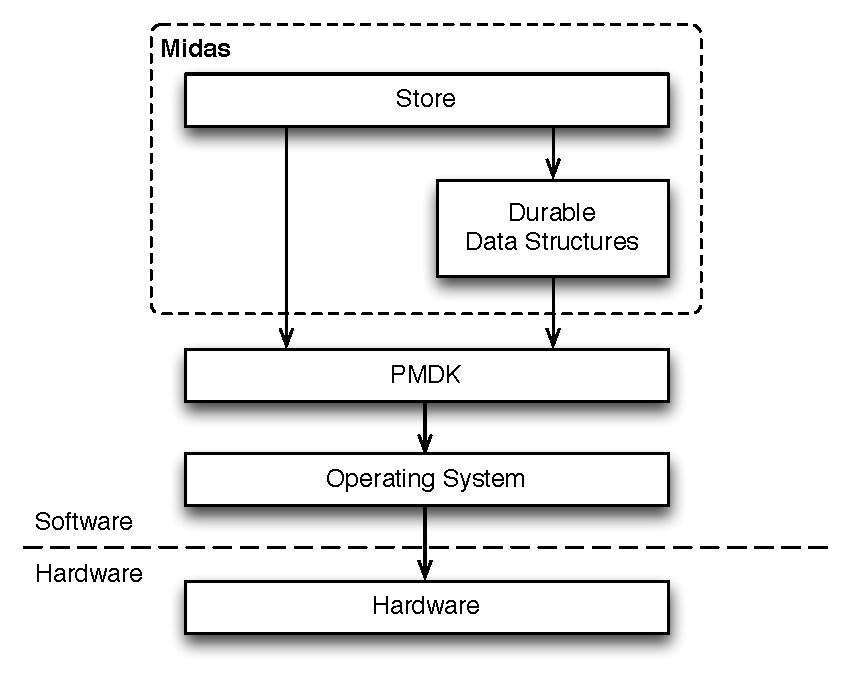
\includegraphics[scale=0.75]{figures/impl/arch2.pdf}
    \caption{System architecture layers of Midas.}
    \label{fig:impl-arch}
\end{figure}

\paragraph{Overview}

Section \ref{ch:impl-nvram} introduces PMDK and shows how it can be used to
access and manage NVRAM. Based on the programming model provided by PMDK, Section
\ref{ch:impl-data} presents the design of two containers classes that are used
to handle data in NVRAM more efficiently. Finally, Section \ref{ch:impl-mvcc}
provides details on transaction management and the serializable MVCC protocol.

\subsection{NVRAM Management}
\label{ch:impl-nvram}

As explained in Chapter \ref{ch:nvram} there are several challenges to the
integration of NVRAM into current systems. Among these are the following:

\begin{itemize}
    \item Accessing NVRAM
    \item Programming against NVRAM
    \begin{itemize}
        \item Separation of volatile from non-volatile data
        \item Recovery of non-volatile objects after restart
        \item Preserving consistency across restarts
    \end{itemize}
\end{itemize}

In the past, several approaches have been discussed to address these challenges.
Recent research, however, shows rising interest in PMDK (formerly known as
NVML). PMDK is a set of both C and C++ libraries and appears to be the first
practical holistic approach to managing NVRAM. Therefore, this work uses PMDK to
implement NVRAM management.

\subsubsection{NVRAM Access}

In PMDK, NVRAM is accessed via ordinary file systems such as \code{ext4} or
\code{tmpfs}. That way, NVRAM can be mapped into a process' address space via
plain files. Using the kernel feature \ac{DAX} file,
systems can bypass the operating system's page cache \cite{oukid2017data,
andrei2017sap, rudoff2017persistent}. This enables true load and store
semantics. In addition, swapping is disabled for the respective memory region.

\subsubsection{Programming Model}

Apart from its core, the essential part of PMDK used in this work is called
\code{pmemobj}. With it, a persistent object pool holds all data that are meant
to be durable. Memory inside the object pool is managed by a designated memory
allocator. For each object which is meant to be durable, it allocates the
required amount of memory and registers the resulting object in the object pool.
This way, all objects can be recovered on restart. From a programmer
perspective, objects are managed in a graph rooted in the object pool. Using
this graph, which is recovered after restart, the programmer can access all
previously durable objects.

\paragraph{Durable Data}

In order to separate volatile from non-volatile objects, there are templated
wrapper classes to manage integral values and dynamically allocated objects:

\begin{itemize}
    \item \code{pmdk::p<T>} for durable integral values
    \item \code{pmdk::persistent\_ptr<T>} for pointers to durable objects
\end{itemize}

\paragraph{Durable Objects and Pointers}

A \code{persistent\_ptr} consists of a non-volatile unique object id and a
virtual memory address within the object pool. The virtual address is volatile
because it is not valid across restarts. Therefore, the object id is mapped to a
relative memory address within the object pool. Using the object id, the virtual
memory address of an object can be computed from its relative address to the
pool base on every restart. This is necessary, because in most operating systems
virtual address space layout is different for each session. When creating an
object, the function \code{pmdk::make\_persistent<T>()} is used. The lifetime of
a durable object spans across scopes and restarts. In order to deallocate an
object, the function \code{pmdk::delete\_persistent<T>()} must be used.

\paragraph{Preserving Consistency}

In order to ensure consistency across crashes in NVRAM, stores must be flushed
immediately. In PMDK, this can be done explicitly for selected memory regions or
implicitly by using a so-called transaction. A transaction receives the current
object pool and a functor. Each persistent property or pointer that is modified
by the functor, registers itself with the transaction. When the transaction
commits, all registered objects are made durable in NVRAM. A transaction commits
when its functor completes without errors. In the example below a durable object
of type \code{T} is created inside a pool which has a graph root of type
\code{Root} (see Listing \ref{lst:pmdk-tx}). Assume the global variable
\code{objCount} is supposed to reflect the correct number of durable objects.
For that purpose, both creating of objects and incrementing the counter are
consolidated in a transaction to form a single memory update.

\begin{figure}[h!]
\begin{lstlisting}
#include "libpmemobj++/persistent_ptr.hpp"
#include "libpmemobj++/transaction.hpp"
#include "libpmemobj++/pool.hpp"
namespace pmdk = pmem::obj;

pmdk::p<size_t> objCount = 0;

template <class T, class Root>
pmdk::persistent_ptr<T> create(pmdk::pool<Root> pop)
{
    pmdk::persistent_ptr<T> obj = nullptr;

    // Consolidate updates in transaction
    pmdk::transaction::exec_tx(pop, [&, this](){
         obj = pmdk::make_persistent<T>();
         objCount = objCount + 1;
    });

    // At this point, all changes to NVM are either completely durable or absent
    return obj;
}
\end{lstlisting}
\caption{Consistent updates to NVM using PMDK transactions.}
\label{lst:pmdk-tx}
\end{figure}

Even though object creation is always transactional in PMDK, initialization is
not. Instead, the memory of an object is only nulled. As a result, each class
intended for durability must be \emph{trivially default constructible}, which
means that a compiler-generated default constructor must be sufficient to
initialize an instance of the class. Otherwise, the programmer has to use custom
initialization procedures.

Internally, PMDK uses largely the same mechanism for consistency as described in
Chapter \ref{ch:nvram-consistency}. That means, modified data are flushed from
memory order buffers and caches. In some situations, non-temporal writes are
used which make use of write combine buffers. When it comes to flushing
write-pending queues inside the memory controller, PMDK relies on ADR.

% =============================================================================
% =============================================================================
% =============================================================================

\subsection{Durable Data Structures}
\label{ch:impl-data}

% The implementation of Midas relies on several classic data structures, such as
% arrays, lists, and hash maps. Since Midas is divided in two separate volatility
% domains, each one requires its own dedicated data structures. While the volatile
% part of Midas is composed of containers from the C++ standard library, the
% non-volatile part is based on custom reimplanations for NVRAM. This section
% outlines the design of durable data structures in Midas. The next section then
% deals with special data structures related to MVCC.

The implementation of Midas relies on several fundamental data structures, such
as arrays, lists, and hash maps. Since Midas is divided in two separate
volatility domains, each one requires its own dedicated data structures. The
volatile part of Midas is composed of containers from the C++ standard library.
The non-volatile part, on the other hand, is based on custom container
implementations using PMDK. This section outlines the design of durable data
structures in Midas.

% In the non-volatile domain of Midas, data structures must be NVRAM-aware. That
% means, that data structures must be recoverable from a durable state when Midas
% starts and also ensure that updates to NVRAM do not cause inconsistencies.

Durable data structures in Midas are the index and the version histories
contained therein. The index is used to lookup version histories, thus it is
implemented as a hash table. Histories, on the other hand, are implemented as
linked lists because they are accessed in linear order. Lacking general-purpose
container libraries based on PMDK, both non-volatile data structures are
developed from scratch.

% \paragraph{Doubly-Linked List}
\subsubsection{Doubly-Linked List}

The doubly-linked list is implemented in the template class \code{NVList}. Its
attributes consist of a pointer to first element, a pointer to the last element,
and an element counter. All these attributes must be durable in order to recover
the list after a restart. Therefore, they are declared as persistent pointers or
properties in terms of PMDK. The API of \code{NVList} is closely related to the
C++ standard library containers. It also provides iterator facilities for
traversal.

\begin{figure}[h!]
    \centering
    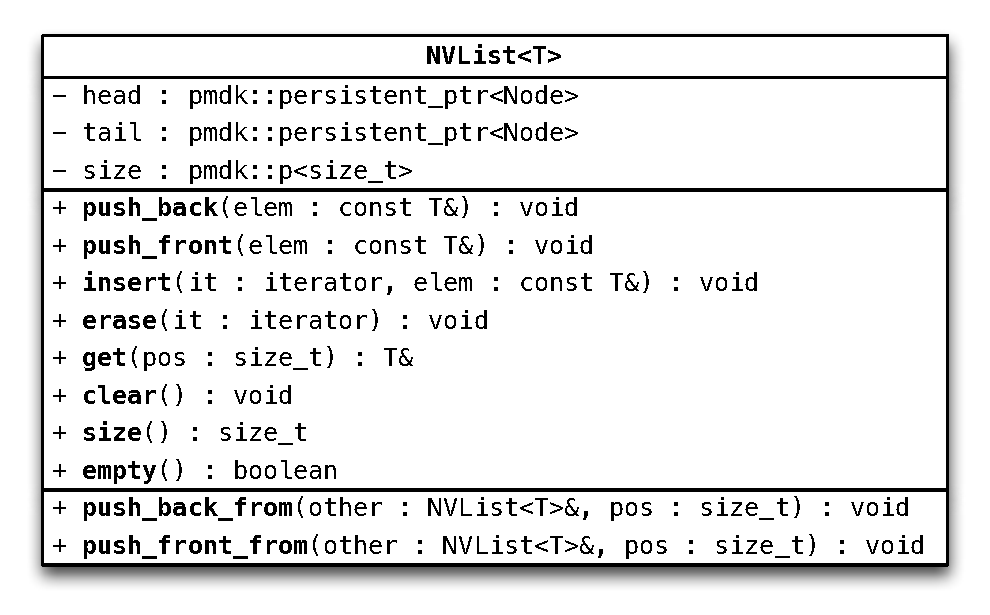
\includegraphics[scale=0.66]{figures/impl/list.pdf}
    \caption{Class diagram for the class \code{NVList}}
    \label{fig:impl-list}
\end{figure}

An important aspect of implementing durable data structures is to preserve
consistency. This is done by consolidating related allocations and operations on
durable objects in a transaction as shown in Chapter \ref{ch:impl-nvram}.

\begin{figure}[h!]
\begin{lstlisting}
void push_back(const elem_type& elem)
{
    pmdk::transaction::exec_tx(pool, [&,this](){
        auto new_node = pmdk::make_persistent<node>();
        new_node->mValue = elem;
        append(new_node);
        mSize = mSize + 1;
    });
}
\end{lstlisting}
\caption{Implementation of \code{push\_back()} as an example for transactional updates to NVRAM}
\label{lst:impl-list-tx}
\end{figure}

An additional feature of \code{NVList} is a zero-copy mechanism for migrating
individual list nodes between different lists. This is useful when nodes from a
single list must be scattered to several other lists as is done when rehashing a
hash table. The feature is provided by the functions \code{push\_back\_from()}
and \code{push\_front\_from()}.

% \paragraph{Hash Table}
\subsubsection{Hash Table}

The hash table is implemented as a template class called \code{NVHashmap}.
Essentially, the table consists of a single persistent array that is reallocated
as needed. Each cell in the index is called slot or bucket. As with
\code{NVList}, the API of \code{NVHashmap} is closely aligned to the C++
standard library. Also, the class employs a policy-based template design which
allows changing its behavior through template parameters.

\begin{figure}[h!]
    \centering
    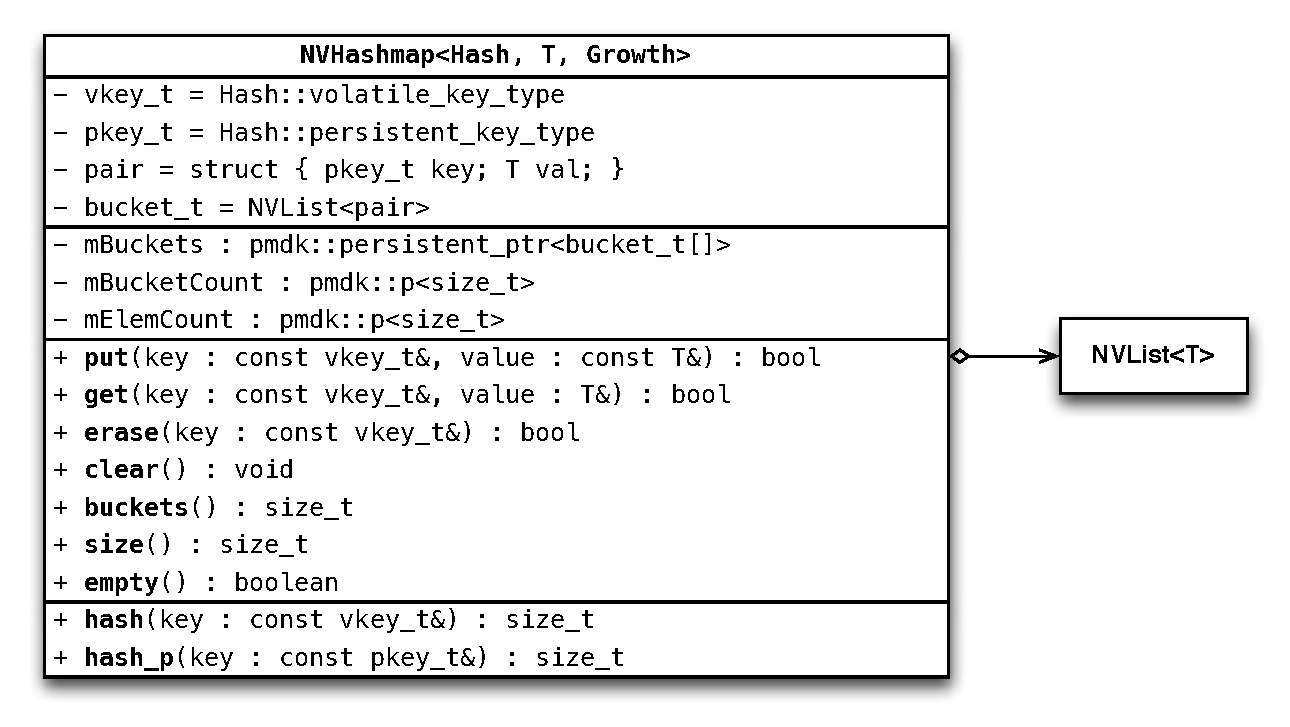
\includegraphics[scale=0.66]{figures/impl/map.pdf}
    \caption{Class diagram for the class \code{NVHashmap}}
    \label{fig:impl-map}
\end{figure}

There are three important aspects to the design of hash tables: the hash
function itself, collision handling, and growth policy. The hash function used
in Midas is a variant of the hash function used in the string library of Java
\cite{javadoc2018hashcode}, which is a polynomial of prime powers and character
bytes as coefficients. The final access index is computed modulo of the current
table size.

When disjoint keys result in equal hashes a collision occurs. In the case of
Midas, collisions are handled by \emph{chaining}. With chaining, each slot in
the table is a linked list and keys are always stored in pairs with their mapped
value. When hashing a key, the corresponding bucket is searched for a pair with
a matching key. If no such pair is found, then the given pair can be inserted.
As a result, each bucket only contains pairs with conflicting key hashes. Both
the collision lists and the pairs are durable.

Because searching long buckets increases access time, the table is expanded
regularly. More precisely, expansion occurs when the maximum load factor is
exceeded. The load factor is defined as the ratio of the number of pairs and the
number of buckets. The maximum load factor is set to $0.75$. In order to
amortize the cost of reallocations, the table size is doubled on each expansion.
After an expansion, all pairs are rehashed into the new table. This is where the
zero-copy list node migration of \code{NVList} is used. Parameters such as the
maximum load factor or the growth factor can be adjusted using the policy-based
template design.

\todo[inline]{impl: elaborate on volatile/non-volatile key dissonance (optional)}

% * policy-based design for
%     * hashing volatile and non-volatile keys
%         * user does not know about a different represent. of obj. in pmem
%         * volatile keys must have equal hashes with non-volatile counterparts
%         * for safety many hash functions are not equal across restarts
%             * => cannot find pairs after restart
%             * => a) use fixed hash function (impl. from JDK)
%             * => b) rehash entire table (expensive!)

% =============================================================================
% =============================================================================
% =============================================================================

\newpage

\subsection{Transaction Management}
\label{ch:impl-mvcc}

This section presents an outline of the transaction management in Midas.

% \subsubsection{Transactions}
\subsubsection{Components}

Transaction management relies on two key data structures: transaction control blocks and the transaction table. This section documents the implementation of these structures.

\todo[inline]{This section now deals with all components, not just transactions}

\paragraph{Transaction Control Blocks}

Transactions are represented by transaction control blocks (TCBs). A TCB holds a unique transaction id (TID), a status code, two timestamps, as well as read and write sets. For historical reasons, a TCB is internally denoted as a \code{Transaction} (see Figure \ref{fig:tcb}).

\begin{figure}[h!]
    \centering
    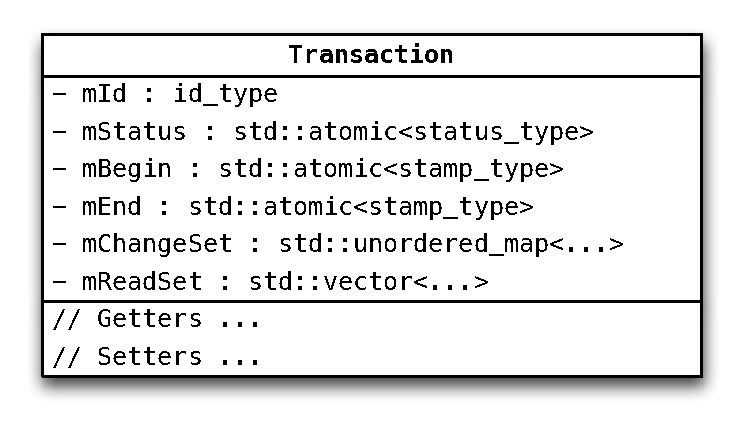
\includegraphics[scale=.75]{figures/impl/tx.pdf}
    \caption{A transaction control block.}
    \label{fig:tcb}
\end{figure}

The TID is required to lookup the associated transaction. The status code indicates the current execution phase of a transaction and can be one of the following:

\begin{itemize}
    \item Active
    \item Failed
    \item Committed
\end{itemize}

The execution phase of a transaction $T$ is used by other transactions to determine $T$'s state if they encounter dirty versions of $T$. In addition, there are two timestamps that denote when $T$ started and when it ended. This information is vital to determine if the lifetimes of two transactions overlap. Since both transaction state and timestamps must be accessible and consistent to transactions from other threads, they are implemented as atomic variables.

When a transaction modifies the store with calls to \code{Store::put()} or \code{Store::drop()}, a designated change entry is stored in the associated TCB. Depending on the operation performed, a change entry contains the following items:

\begin{itemize}
    \item an operation descriptor
    \item a pointer to the original version
    \item the raw updated value
    \item a pointer to the updated version
\end{itemize}

Based on the operation descriptor, knows how to perform the change. For instance, if the change resulted from a \code{Store::drop()}, then it only contains a pointer to the original version which has to be invalidated. Change sets are implemented as hash tables. This is because a transaction might update an item multiple times and looking up a previously written item is faster than repeatedly scanning an item's history. In order to detect read-write conflicts, and thus enable serializability, a TCB also has to record all items that were read. Because read sets can grow large in read-mostly environments, they are implemented as dynamic arrays to amortize allocation cost. Both read and change sets are thread local storage and are therefore not synchronized.

When a transaction is started with \code{Store::begin()}, a TCB is created. During initialization the TCB is assigned a TID and a start timestamp.  Once the TCB is initialized, its TID is used as a key to insert it into the transaction table. The lifetime of a TCB, including its transaction, ends when it is removed from the transaction table. This happens when the associated transaction encounters a conflict or is aborted with \code{Store::abort()}.

\todo[inline]{add algorithm listing?}

\paragraph{TIDs and Timestamps}

TIDs and timestamps are represented by 64-bit unsigned integers. They are acquired by incrementing a designated global counter, respectively. In order to ensure that the counters are consistent across all cores, they are incremented using atomic fetch-and-add instructions. Because there are situations where TIDs and timestamps must be distinguished from another, their value ranges are interleaved. TIDs are always odd numbers, whereas timestamps are always even. Each counter is incremented by two, accordingly. The reason for this design is explained in the next section.

\paragraph{Transaction Table}

As explained above, there are situations when transactions may need to determine the state of other concurrent transactions. Therefore, TCBs are stored in a global transaction table. In order to provide fast lookup, the transaction table is implemented as a hash table. Each TCB is hashed using its TID. However, the table is a globally shared resource that must be synchronized. In order to prevent a bottleneck, the concurrent hash table implementation \emph{libcuckoo} is used \cite{fan2013memc3, li2014algorithmic, libcuckoo2018home}.

\paragraph{Versions}

With MVCC, concurrent access to data is managed by having multiple versions of an item. In this case, the value of each key-value pair is versioned. In Midas, a version is durable and consists of the actual data value and two timestamps indicating the lifetime of the version. The data value is represented by a durable dynamic array of characters, similar to \code{std::string} from the C++ standard library. Because all transactions must have a consistent view on the lifetime of a version, its timestamps are only accessed by means of atomic instructions. The timestamp fields can be used in several ways, as shown in the next section.

\paragraph{Histories}

For each value of a key-value pair, there are several versions. The versions of a single item are managed within a history. When a transaction wishes to access an item, the transaction management has to search the item's history for version that is \emph{visible} to the transaction. In Midas, a history is a durable linked list by means of \code{NVList} from Section \ref{ch:impl-data}. At startup, existing histories are truncated to contain only their most recent version. After that, histories are in append-only mode.

\paragraph{Index}

Another core data structure in Midas is the index. It accomplishes the mapping between the key of an item and the item's version history. Whenever a transactional operation wishes to access an item, it has to query the index with the corresponding key. The index must provide fast lookup and is therefore implemented as a hash table. For that purpose, the durable hash table \code{NVHashmap} from Section \ref{ch:impl-data} is used. The index is accessed by all concurrent transactions and must therefore be synchronized. Due to the complexity of concurrent data structure design, a lock is used to protect the index. This is likely to become a serious bottleneck and should be revised in future work.

\subsubsection{Transaction Processing}

Unlike other \acp{KVS}, Midas can only be operated through transactions. Transactions that are either terminated or were not created by the respective store instance are rejected. Once a transaction has been started, it can be used to modify the store with the following operations:

\begin{itemize}
    \item \code{read(tx, <key>, <result>)}
    \item \code{write(tx, <key>, <value>)}
    \item \code{drop(tx, <key>)}
\end{itemize}

In general, the control flow of these operations is structured in the same way. At first the operation checks its inputs for errors. Next, it looks up the history of the item associated with the specified key.

\paragraph{Visibility}

\paragraph{Conflicts}

\paragraph{Commits}
